\nonstopmode
\documentclass[10pt, a4paper]{article}
\parindent=20pt
\parskip=8pt
\usepackage[width=15.5cm, left=3cm, top=2.5cm, height= 24.5cm]{geometry}
\usepackage[spanish]{babel}
\usepackage[utf8]{inputenc}
\usepackage{fancyhdr}
\usepackage{multirow}
\usepackage{rotating}
\usepackage{indentfirst}
\usepackage{latexsym}
\usepackage{caratula}
\usepackage{gnuplottex}
\usepackage{epsfig}
\usepackage{lastpage}
\usepackage{amsfonts}
\usepackage{listings}
\lstset{language=C}
%\usepackage[export]{adjustbox}
\usepackage{pdfpages}
\usepackage{amsmath}
\usepackage{verbatim}
%\usepackage[ruled,vlined,linesnumbered]{algorithm2e}
\usepackage{graphicx}
\usepackage{float}
\usepackage{color}

\graphicspath{{imgs/}}

% Acomodo fancyhdr.
\pagestyle{fancy}
\thispagestyle{fancy}
\addtolength{\headheight}{1pt}
\lhead{Teor\'ia de las Comunicaciones}
\rhead{TP1}
\cfoot{\thepage /\pageref{LastPage}}
\renewcommand{\footrulewidth}{0.4pt}
\renewcommand{\thesubsubsection}{\thesubsection.\alph{subsubsection}}


\author{Teor\'ia de las Comunicaciones, DC, UBA.}
\date{}
\title{}

\begin{document}
	
\thispagestyle{empty}
\materia{Teor\'ia de las Comunicaciones}
%\submateria{Trabajo Pr\'actico Nº1}
\titulo{Trabajo Práctico Nº1}
\integrante{Rivero, Maximiliano}{366/07}{maxirivero088@gmail.com}
\integrante{Izcovich, Sabrina}{550/11}{sizcovich@gmail.com}
\integrante{Rogani, Marcos}{520/05}{marcos.rogani@gmail.com}

\maketitle

\tableofcontents
\newpage

\section{Introducción}
El objetivo del trabajo práctico consistió en analizar estadísticamente el protocolo de comunicación ARP\footnote{Protocolo de Red de bajo nivel para traducir direcciones IP en direcciones MAC donde se encuentran direcciones IP de capa 3 con direcciones MAC de capa 2.} de un segmento de red determinado. Con este fin, se elaboraron mediciones en distintos espacios de redes públicas para estudiar la entropía de cada una de ellas en base a los mensajes ARP observados.

ARP (Address Resolution Protocol) consiste en un protocolo usado frecuentemente por las redes locales para conectar las capas 3 (capa de red) y 2 (capa de enlace) mediante la conversión o identificación de IP v4 con direcciones físicas MAC.

Los dos tipos de paquetes posibles en dicho protocolo son los paquetes de petición y de respuesta:
\begin{itemize}
\item Los paquetes de petición ($who-has$) son enviados mayormente en forma de broadcast con el objetivo de poder localizar la dirección MAC a la cual le pertenece una IP conocida.
\item Los paquetes de respuesta ($is-at$) son enviados de manera unicast pues se utilizan para responder a la máquina que realizó una petición con anterioridad.
\end{itemize}

Los paquetes ARP consisten de los siguientes campos:
\begin{itemize}
\item Operación: Especifica la operación que el emisor está realizando. 1 para petición, 2 para responder.
\item Dirección MAC del emisor.
\item Dirección IP del emisior.
\item Dirección MAC del destinatario: Este campo se ignora en las peticiones.
\item Dirección IP del destinatario.
\end{itemize}
\begin{figure}[H] %[h] Aqui [b] para button [t] para top
\begin{center}
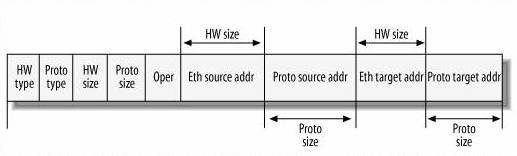
\includegraphics[width=350pt]{../imgs/arp.jpg}
\caption{Formato de una ARP.}
\end{center}
\end{figure}

Un ejemplo típico de uso podría ser el siguiente:\newline

\begin{quotation}
Una máquina en una red desea enviarle un paquete de datos a otra máquina de la misma red. Para eso, la máquina emisora busca, en su tabla local, la dirección MAC asociada a la dirección IP a la cuál desea mandar el paquete. Si no la encuentra, realiza el broadcast de la petición ARP, que llegará eventualmente si se encuentra conectada, a la máquina destino. 
La máquina destino recibirá la petición y responderá de manera unicast a la máquina que realizó la petición, poniendo en el paquete su dirección MAC para que la máquina destino de la respuesta pueda conocer la dirección MAC que necesitaba.
\end{quotation}

El análisis de la red consiste en reconocer su topología en base al nivel de información que proveen las diferentes IP, como fuente y como destino, tomando a las IP como símbolos y estimado su probabilidad de aparición con su frecuencia muestral. Para nuestro análisis, nos limitamos a la utilización de los paquetes $who-has$.

\section{Desarrollo}

Con el fin de obtener resultados relevantes, decidimos analizar redes Wi-Fi públicas de gran uso. Éstas fueron:

\begin{itemize}
\item CECEN-Wifi - Red pública del Pabellón II de Ciudad Universitaria, de gran utilización por parte de los estudiantes y docentes de la facultad.
\item Starbucks Núñez - Red pública utilizada por los clientes.
\item Red Empresarial - Con una magnitud aproximada de 30 dispositivos conectados en simultáneo.
\end{itemize}

Los tiempos de captura fueron los siguientes:

\begin{center}
  \begin{tabular}{| l | c |}
    \hline
    CECEN-Wifi & 23 minutos\\ \hline
    Starbucks & 3 horas\\ \hline
    Red Empresarial & 30 minutos\\
    \hline
  \end{tabular}
\end{center}

Para la captura de paquetes, generamos un script que, a partir de Scapy\footnote{http://www.secdev.org/projects/scapy/}, $sniffeara$ la red y almacenara las IP's fuente y destino involucradas en el envío y recepción de paquetes. Para corroborar la correctitud de nuestros datos, utilizamos Wireshark\footnote{http://www.wireshark.org} y comparamos lo obtenido con los resultados del programa. 

Para almacenar los resultados, filtramos por redes ARP y $who-has$. Los resultados obtenidos fueron los siguientes:

\section{Resultados}
Con el fin de visualizar los intercambios de paquetes obtenidos, utilizamos $yED$\footnote{http://www.yworks.com/en/products\_yed\_about.html} para realizar gráficos adecuados para ello. Para esto, decidimos presentarlos en forma de grafos dirigidos de IPs con pesos en los nodos (donde existe un eje entre la IP $x$ y la IP $y$ sí y sólo sí se observó un request ARP con source IP $x$ y target IP $y$). Para eso, modificamos su formato obtenido de la forma $IP_{src}\ IP_{dst}$.

Los resultados obtenidos fueron los siguientes:

\subsection{CECEN-Wifi}

La red del $CECEN$ fue capturada durante 23 minutos. Los intercambios que se realizaron en ese tiempo fueron los que se pueden ver a continuación:
\begin{figure}[H] %[h] Aqui [b] para button [t] para top
\begin{center}
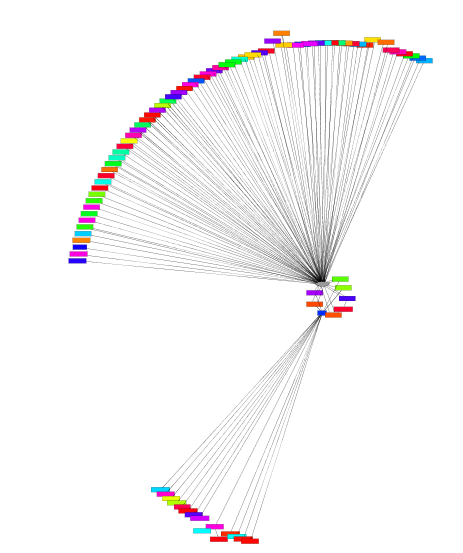
\includegraphics[width=400pt]{../imgs/cecen_entero.png}
\caption{Resultado de la captura de envío y recepción de paquetes de la red CECEN-Wifi.}
\end{center}
\end{figure}

\begin{figure}[H] %[h] Aqui [b] para button [t] para top
\begin{center}
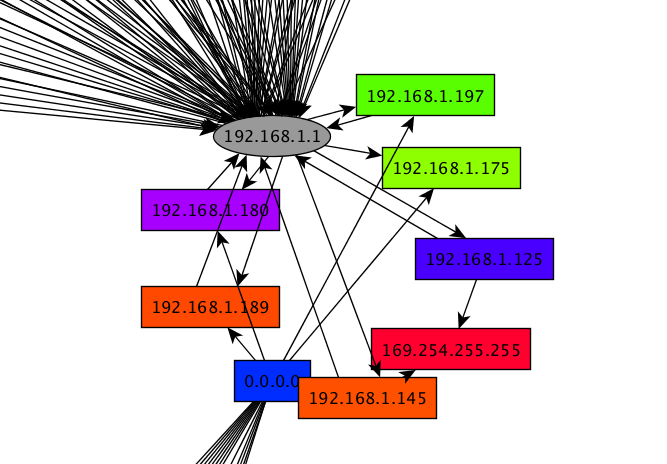
\includegraphics[width=400pt]{../imgs/cecen_centro.png}
\caption{Resultado de la captura de envío y recepción de paquetes de la red CECEN-Wifi.}
\end{center}
\end{figure}

\begin{figure}[H] %[h] Aqui [b] para button [t] para top
\begin{center}
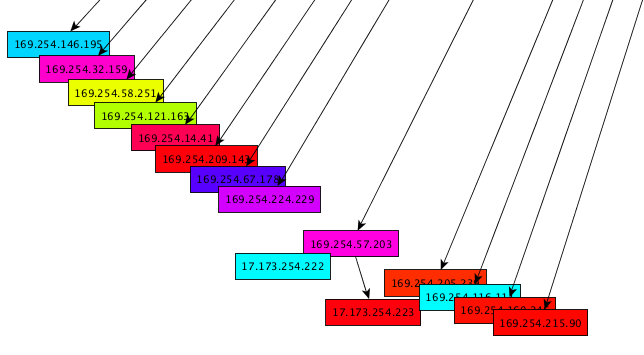
\includegraphics[width=400pt]{../imgs/cecen_costado.png}
\caption{Resultado de la captura de envío y recepción de paquetes de la red CECEN-Wifi.}
\end{center}
\end{figure}

\begin{figure}[H] %[h] Aqui [b] para button [t] para top
\begin{center}
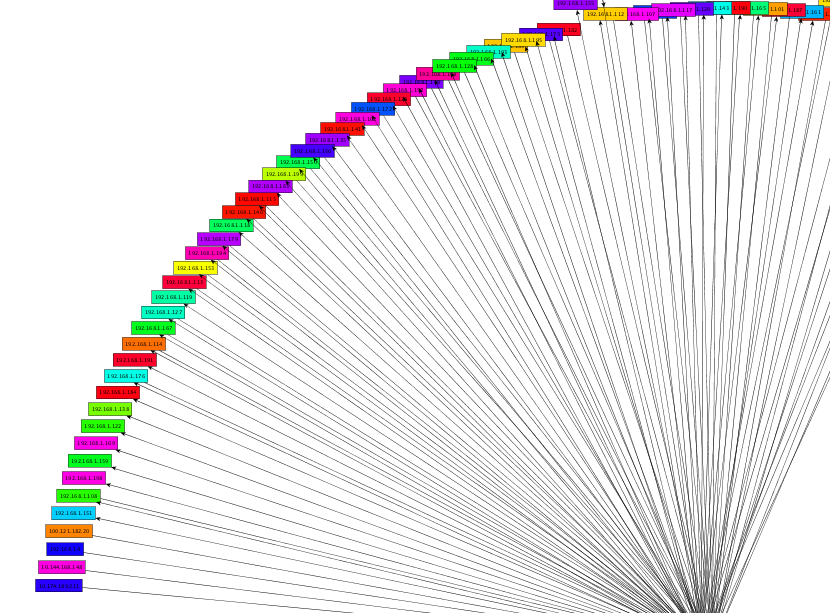
\includegraphics[width=400pt]{../imgs/cecen_arriba.png}
\caption{Resultado de la captura de envío y recepción de paquetes de la red CECEN-Wifi.}
\end{center}
\end{figure}

\subsection{Starbucks}

La medición realizada durante 3 horas dio el siguientes resultado:
\begin{figure}[H] %[h] Aqui [b] para button [t] para top
\begin{center}
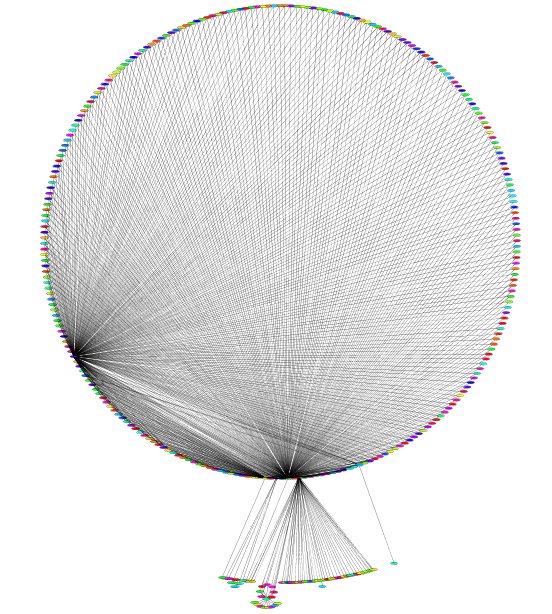
\includegraphics[width=400pt]{../imgs/starbucks_entero.png}
\caption{Resultado de la captura de envío y recepción de paquetes de Starbucks durante tres horas.}
\end{center}
\end{figure}

Con el fin de lograr extraer conclusiones relevantes sobre el intercambio de paquetes en dicha red, acotamos el tiempo de captura a 30 minutos. El resultado fue el que sigue:

\begin{figure}[H] %[h] Aqui [b] para button [t] para top
\begin{center}
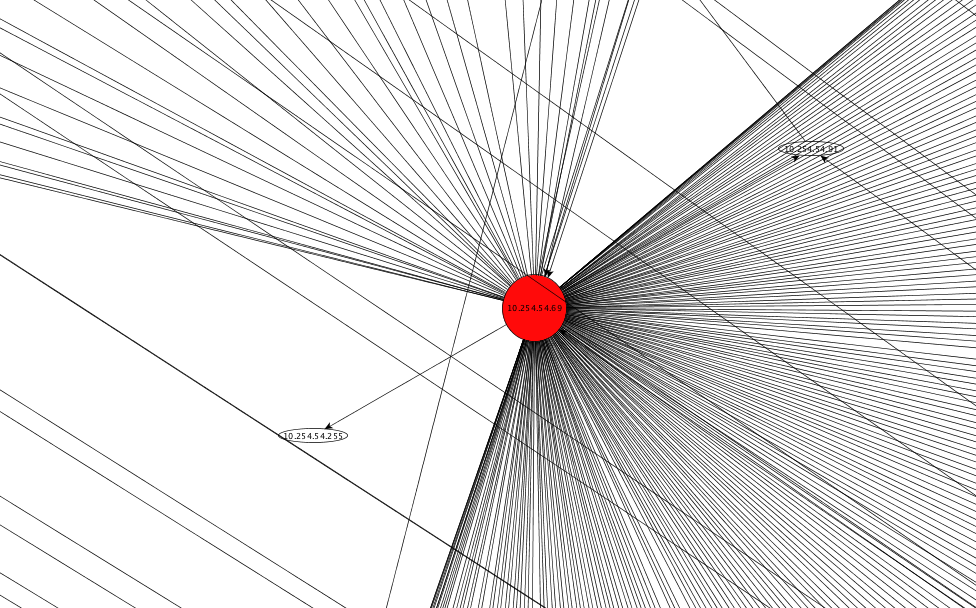
\includegraphics[width=400pt]{../imgs/starbucks30_1.png}
\caption{Resultado de la captura de envío y recepción de paquetes de Starbucks durante tres horas.}
\end{center}
\end{figure}

\begin{figure}[H] %[h] Aqui [b] para button [t] para top
\begin{center}
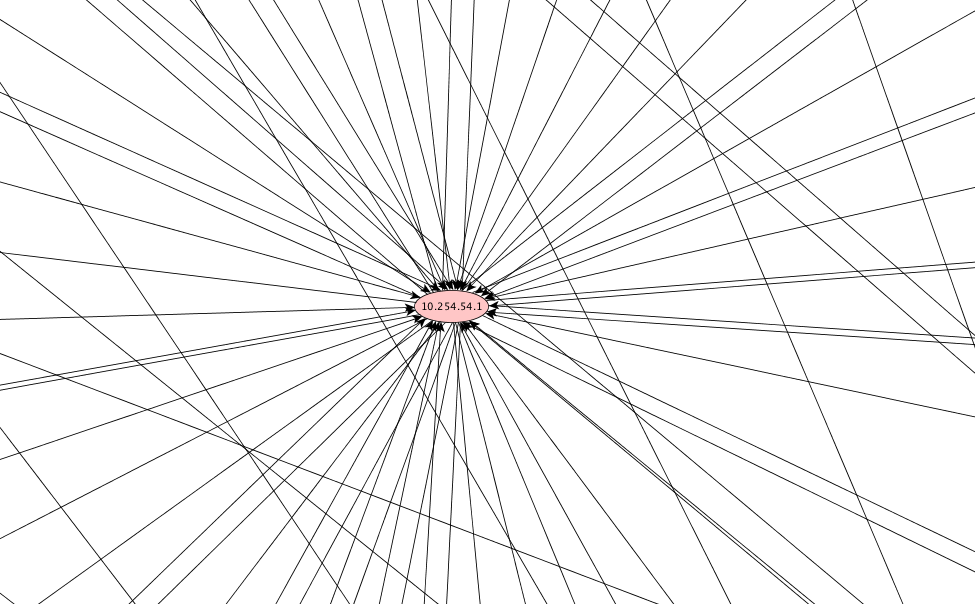
\includegraphics[width=400pt]{../imgs/starbucks30_2.png}
\caption{Resultado de la captura de envío y recepción de paquetes de Starbucks durante tres horas.}
\end{center}
\end{figure}

\begin{figure}[H] %[h] Aqui [b] para button [t] para top
\begin{center}
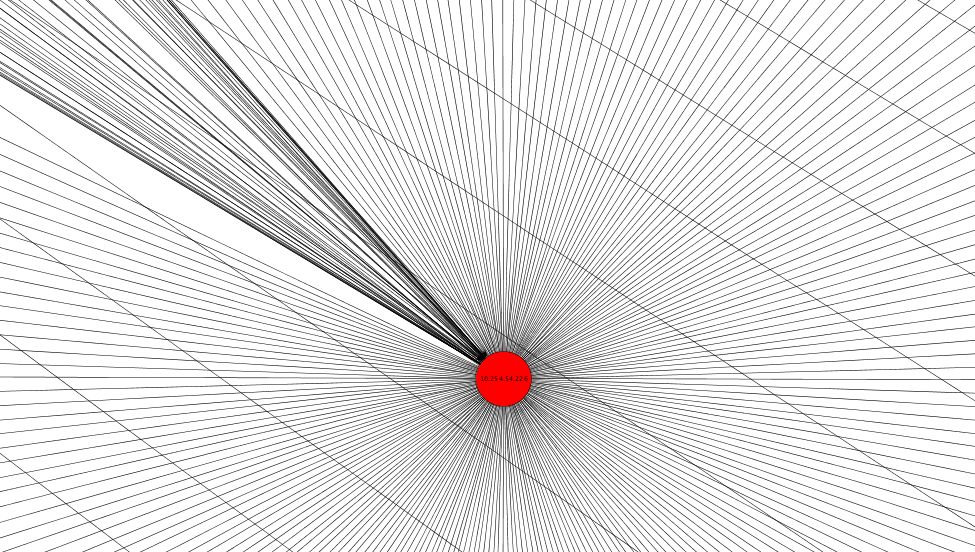
\includegraphics[width=400pt]{../imgs/starbucks30_3.png}
\caption{Resultado de la captura de envío y recepción de paquetes de Starbucks durante tres horas.}
\end{center}
\end{figure}


\subsection{Red Empresarial}


\begin{figure}[H] %[h] Aqui [b] para button [t] para top
\begin{center}
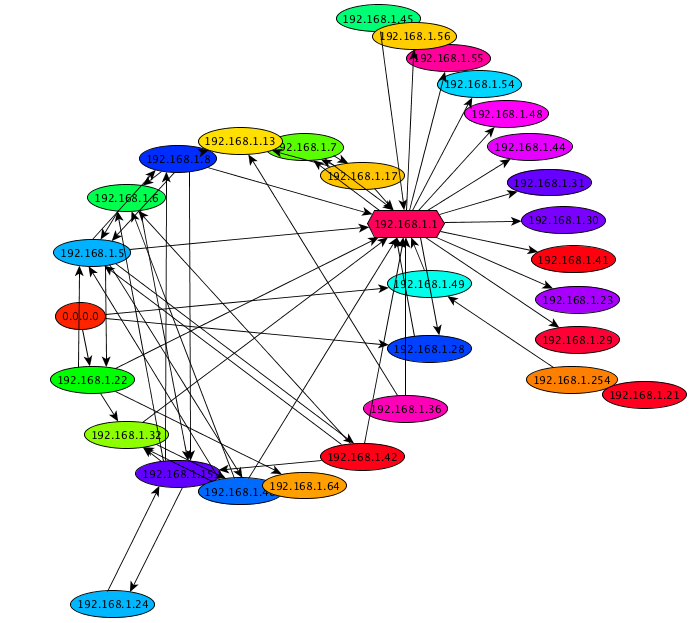
\includegraphics[width=400pt]{../imgs/tiargsa_entero.png}
\caption{Resultado de la captura de envío y recepción de paquetes de una empresa.}
\end{center}
\end{figure}

\subsubsection{Informaci\'on fuente src}
Por otro lado, graficamos los gráficos de barra respecto de la entropía. De este modo, logramos analizar qué IPs son estadísticamente significativas en la LAN analizando la información de cada símbolo con respecto a la entropía de su respectiva fuente.
A continuaci\'on se muestran las 10 ips con menor cantidad de informaci\'on.

%% GNUPLOT: LaTeX picture with Postscript
\begingroup
  \makeatletter
  \providecommand\color[2][]{%
    \GenericError{(gnuplot) \space\space\space\@spaces}{%
      Package color not loaded in conjunction with
      terminal option `colourtext'%
    }{See the gnuplot documentation for explanation.%
    }{Either use 'blacktext' in gnuplot or load the package
      color.sty in LaTeX.}%
    \renewcommand\color[2][]{}%
  }%
  \providecommand\includegraphics[2][]{%
    \GenericError{(gnuplot) \space\space\space\@spaces}{%
      Package graphicx or graphics not loaded%
    }{See the gnuplot documentation for explanation.%
    }{The gnuplot epslatex terminal needs graphicx.sty or graphics.sty.}%
    \renewcommand\includegraphics[2][]{}%
  }%
  \providecommand\rotatebox[2]{#2}%
  \@ifundefined{ifGPcolor}{%
    \newif\ifGPcolor
    \GPcolorfalse
  }{}%
  \@ifundefined{ifGPblacktext}{%
    \newif\ifGPblacktext
    \GPblacktexttrue
  }{}%
  % define a \g@addto@macro without @ in the name:
  \let\gplgaddtomacro\g@addto@macro
  % define empty templates for all commands taking text:
  \gdef\gplbacktext{}%
  \gdef\gplfronttext{}%
  \makeatother
  \ifGPblacktext
    % no textcolor at all
    \def\colorrgb#1{}%
    \def\colorgray#1{}%
  \else
    % gray or color?
    \ifGPcolor
      \def\colorrgb#1{\color[rgb]{#1}}%
      \def\colorgray#1{\color[gray]{#1}}%
      \expandafter\def\csname LTw\endcsname{\color{white}}%
      \expandafter\def\csname LTb\endcsname{\color{black}}%
      \expandafter\def\csname LTa\endcsname{\color{black}}%
      \expandafter\def\csname LT0\endcsname{\color[rgb]{1,0,0}}%
      \expandafter\def\csname LT1\endcsname{\color[rgb]{0,1,0}}%
      \expandafter\def\csname LT2\endcsname{\color[rgb]{0,0,1}}%
      \expandafter\def\csname LT3\endcsname{\color[rgb]{1,0,1}}%
      \expandafter\def\csname LT4\endcsname{\color[rgb]{0,1,1}}%
      \expandafter\def\csname LT5\endcsname{\color[rgb]{1,1,0}}%
      \expandafter\def\csname LT6\endcsname{\color[rgb]{0,0,0}}%
      \expandafter\def\csname LT7\endcsname{\color[rgb]{1,0.3,0}}%
      \expandafter\def\csname LT8\endcsname{\color[rgb]{0.5,0.5,0.5}}%
    \else
      % gray
      \def\colorrgb#1{\color{black}}%
      \def\colorgray#1{\color[gray]{#1}}%
      \expandafter\def\csname LTw\endcsname{\color{white}}%
      \expandafter\def\csname LTb\endcsname{\color{black}}%
      \expandafter\def\csname LTa\endcsname{\color{black}}%
      \expandafter\def\csname LT0\endcsname{\color{black}}%
      \expandafter\def\csname LT1\endcsname{\color{black}}%
      \expandafter\def\csname LT2\endcsname{\color{black}}%
      \expandafter\def\csname LT3\endcsname{\color{black}}%
      \expandafter\def\csname LT4\endcsname{\color{black}}%
      \expandafter\def\csname LT5\endcsname{\color{black}}%
      \expandafter\def\csname LT6\endcsname{\color{black}}%
      \expandafter\def\csname LT7\endcsname{\color{black}}%
      \expandafter\def\csname LT8\endcsname{\color{black}}%
    \fi
  \fi
  \setlength{\unitlength}{0.0500bp}%
  \begin{picture}(9000.00,4500.00)%
    \gplgaddtomacro\gplbacktext{%
      \colorrgb{0.00,0.00,0.00}%
      \put(620,240){\makebox(0,0)[r]{\strut{}0}}%
      \colorrgb{0.00,0.00,0.00}%
      \put(620,1044){\makebox(0,0)[r]{\strut{}2}}%
      \colorrgb{0.00,0.00,0.00}%
      \put(620,1848){\makebox(0,0)[r]{\strut{}4}}%
      \colorrgb{0.00,0.00,0.00}%
      \put(620,2651){\makebox(0,0)[r]{\strut{}6}}%
      \colorrgb{0.00,0.00,0.00}%
      \put(620,3455){\makebox(0,0)[r]{\strut{}8}}%
      \colorrgb{0.00,0.00,0.00}%
      \put(620,4259){\makebox(0,0)[r]{\strut{}10}}%
      \colorrgb{0.00,0.00,0.00}%
      \put(160,2249){\rotatebox{90}{\makebox(0,0){\strut{}Informaci\'on}}}%
    }%
    \gplgaddtomacro\gplfronttext{%
      \colorrgb{0.00,0.00,0.00}%
      \put(1458,29){\rotatebox{45}{\makebox(0,0)[r]{\strut{}192.168.1.1}}}%
      \put(2176,29){\rotatebox{45}{\makebox(0,0)[r]{\strut{}192.168.1.187}}}%
      \put(2894,29){\rotatebox{45}{\makebox(0,0)[r]{\strut{}192.168.1.140}}}%
      \put(3612,29){\rotatebox{45}{\makebox(0,0)[r]{\strut{}0.0.0.0}}}%
      \put(4330,29){\rotatebox{45}{\makebox(0,0)[r]{\strut{}192.168.1.125}}}%
      \put(5049,29){\rotatebox{45}{\makebox(0,0)[r]{\strut{}192.168.1.180}}}%
      \put(5767,29){\rotatebox{45}{\makebox(0,0)[r]{\strut{}192.168.1.157}}}%
      \put(6485,29){\rotatebox{45}{\makebox(0,0)[r]{\strut{}169.254.57.203}}}%
      \put(7203,29){\rotatebox{45}{\makebox(0,0)[r]{\strut{}192.168.1.104}}}%
      \put(7921,29){\rotatebox{45}{\makebox(0,0)[r]{\strut{}192.168.1.116}}}%
    }%
    \gplbacktext
    \put(0,0){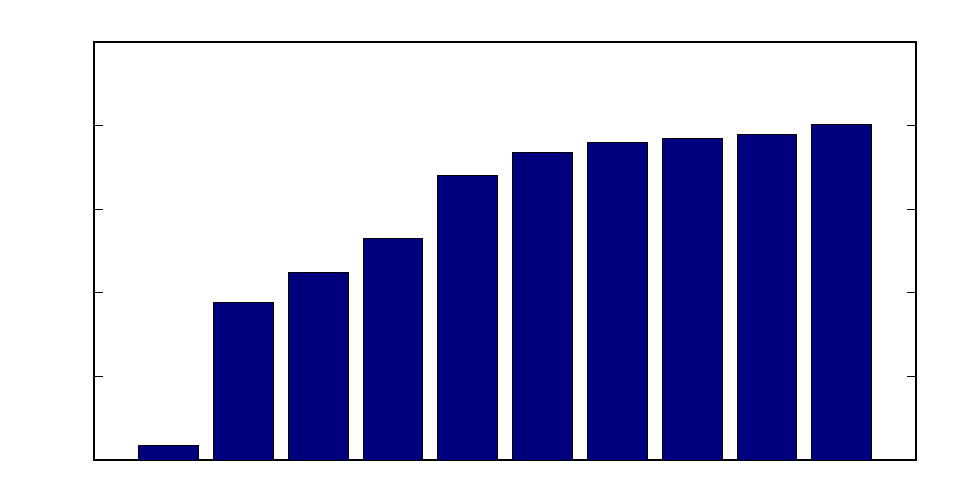
\includegraphics{./imgs/chartBar/cecen_src_barchart}}%
    \gplfronttext
  \end{picture}%
\endgroup

\vspace{2cm}

\subsubsection{Informaci\'on fuente dst}
A continuaci\'on se muestran las 10 ips con menor cantidad de informaci\'on.

%% GNUPLOT: LaTeX picture with Postscript
\begingroup
  \makeatletter
  \providecommand\color[2][]{%
    \GenericError{(gnuplot) \space\space\space\@spaces}{%
      Package color not loaded in conjunction with
      terminal option `colourtext'%
    }{See the gnuplot documentation for explanation.%
    }{Either use 'blacktext' in gnuplot or load the package
      color.sty in LaTeX.}%
    \renewcommand\color[2][]{}%
  }%
  \providecommand\includegraphics[2][]{%
    \GenericError{(gnuplot) \space\space\space\@spaces}{%
      Package graphicx or graphics not loaded%
    }{See the gnuplot documentation for explanation.%
    }{The gnuplot epslatex terminal needs graphicx.sty or graphics.sty.}%
    \renewcommand\includegraphics[2][]{}%
  }%
  \providecommand\rotatebox[2]{#2}%
  \@ifundefined{ifGPcolor}{%
    \newif\ifGPcolor
    \GPcolorfalse
  }{}%
  \@ifundefined{ifGPblacktext}{%
    \newif\ifGPblacktext
    \GPblacktexttrue
  }{}%
  % define a \g@addto@macro without @ in the name:
  \let\gplgaddtomacro\g@addto@macro
  % define empty templates for all commands taking text:
  \gdef\gplbacktext{}%
  \gdef\gplfronttext{}%
  \makeatother
  \ifGPblacktext
    % no textcolor at all
    \def\colorrgb#1{}%
    \def\colorgray#1{}%
  \else
    % gray or color?
    \ifGPcolor
      \def\colorrgb#1{\color[rgb]{#1}}%
      \def\colorgray#1{\color[gray]{#1}}%
      \expandafter\def\csname LTw\endcsname{\color{white}}%
      \expandafter\def\csname LTb\endcsname{\color{black}}%
      \expandafter\def\csname LTa\endcsname{\color{black}}%
      \expandafter\def\csname LT0\endcsname{\color[rgb]{1,0,0}}%
      \expandafter\def\csname LT1\endcsname{\color[rgb]{0,1,0}}%
      \expandafter\def\csname LT2\endcsname{\color[rgb]{0,0,1}}%
      \expandafter\def\csname LT3\endcsname{\color[rgb]{1,0,1}}%
      \expandafter\def\csname LT4\endcsname{\color[rgb]{0,1,1}}%
      \expandafter\def\csname LT5\endcsname{\color[rgb]{1,1,0}}%
      \expandafter\def\csname LT6\endcsname{\color[rgb]{0,0,0}}%
      \expandafter\def\csname LT7\endcsname{\color[rgb]{1,0.3,0}}%
      \expandafter\def\csname LT8\endcsname{\color[rgb]{0.5,0.5,0.5}}%
    \else
      % gray
      \def\colorrgb#1{\color{black}}%
      \def\colorgray#1{\color[gray]{#1}}%
      \expandafter\def\csname LTw\endcsname{\color{white}}%
      \expandafter\def\csname LTb\endcsname{\color{black}}%
      \expandafter\def\csname LTa\endcsname{\color{black}}%
      \expandafter\def\csname LT0\endcsname{\color{black}}%
      \expandafter\def\csname LT1\endcsname{\color{black}}%
      \expandafter\def\csname LT2\endcsname{\color{black}}%
      \expandafter\def\csname LT3\endcsname{\color{black}}%
      \expandafter\def\csname LT4\endcsname{\color{black}}%
      \expandafter\def\csname LT5\endcsname{\color{black}}%
      \expandafter\def\csname LT6\endcsname{\color{black}}%
      \expandafter\def\csname LT7\endcsname{\color{black}}%
      \expandafter\def\csname LT8\endcsname{\color{black}}%
    \fi
  \fi
  \setlength{\unitlength}{0.0500bp}%
  \begin{picture}(9000.00,4500.00)%
    \gplgaddtomacro\gplbacktext{%
      \colorrgb{0.00,0.00,0.00}%
      \put(500,240){\makebox(0,0)[r]{\strut{}0}}%
      \colorrgb{0.00,0.00,0.00}%
      \put(500,1044){\makebox(0,0)[r]{\strut{}1}}%
      \colorrgb{0.00,0.00,0.00}%
      \put(500,1848){\makebox(0,0)[r]{\strut{}2}}%
      \colorrgb{0.00,0.00,0.00}%
      \put(500,2651){\makebox(0,0)[r]{\strut{}3}}%
      \colorrgb{0.00,0.00,0.00}%
      \put(500,3455){\makebox(0,0)[r]{\strut{}4}}%
      \colorrgb{0.00,0.00,0.00}%
      \put(500,4259){\makebox(0,0)[r]{\strut{}5}}%
      \colorrgb{0.00,0.00,0.00}%
      \put(160,2249){\rotatebox{90}{\makebox(0,0){\strut{}Informaci\'on}}}%
    }%
    \gplgaddtomacro\gplfronttext{%
      \colorrgb{0.00,0.00,0.00}%
      \put(1349,29){\rotatebox{45}{\makebox(0,0)[r]{\strut{}192.168.1.1}}}%
      \put(2078,29){\rotatebox{45}{\makebox(0,0)[r]{\strut{}192.168.1.165}}}%
      \put(2807,29){\rotatebox{45}{\makebox(0,0)[r]{\strut{}192.168.1.128}}}%
      \put(3536,29){\rotatebox{45}{\makebox(0,0)[r]{\strut{}192.168.1.153}}}%
      \put(4265,29){\rotatebox{45}{\makebox(0,0)[r]{\strut{}192.168.1.105}}}%
      \put(4994,29){\rotatebox{45}{\makebox(0,0)[r]{\strut{}192.168.1.116}}}%
      \put(5723,29){\rotatebox{45}{\makebox(0,0)[r]{\strut{}192.168.1.197}}}%
      \put(6452,29){\rotatebox{45}{\makebox(0,0)[r]{\strut{}192.168.1.122}}}%
      \put(7181,29){\rotatebox{45}{\makebox(0,0)[r]{\strut{}192.168.1.127}}}%
      \put(7910,29){\rotatebox{45}{\makebox(0,0)[r]{\strut{}192.168.1.139}}}%
    }%
    \gplbacktext
    \put(0,0){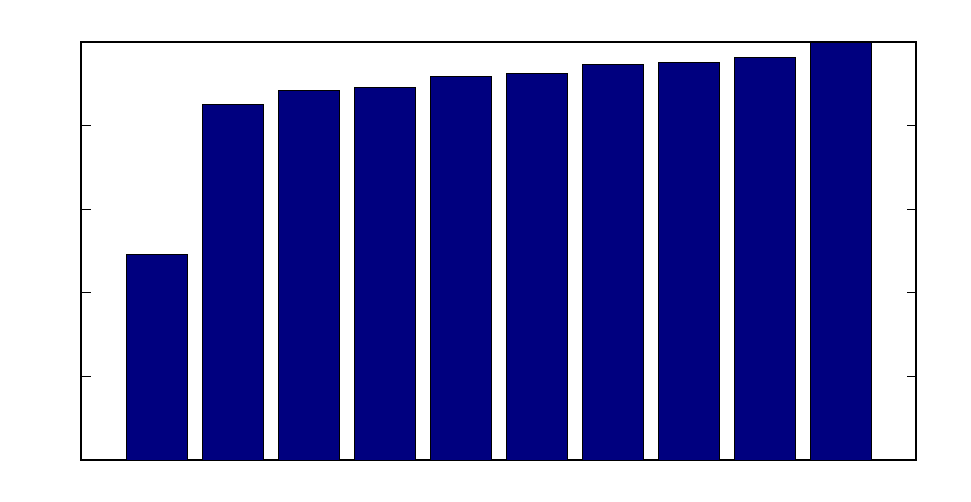
\includegraphics{./imgs/chartBar/cecen_dst_barchart}}%
    \gplfronttext
  \end{picture}%
\endgroup

\vspace{2cm}


\subsubsection{Informaci\'on fuente src}
A continuaci\'on se muestran las 10 ips con menor cantidad de informaci\'on.

%% GNUPLOT: LaTeX picture with Postscript
\begingroup
  \makeatletter
  \providecommand\color[2][]{%
    \GenericError{(gnuplot) \space\space\space\@spaces}{%
      Package color not loaded in conjunction with
      terminal option `colourtext'%
    }{See the gnuplot documentation for explanation.%
    }{Either use 'blacktext' in gnuplot or load the package
      color.sty in LaTeX.}%
    \renewcommand\color[2][]{}%
  }%
  \providecommand\includegraphics[2][]{%
    \GenericError{(gnuplot) \space\space\space\@spaces}{%
      Package graphicx or graphics not loaded%
    }{See the gnuplot documentation for explanation.%
    }{The gnuplot epslatex terminal needs graphicx.sty or graphics.sty.}%
    \renewcommand\includegraphics[2][]{}%
  }%
  \providecommand\rotatebox[2]{#2}%
  \@ifundefined{ifGPcolor}{%
    \newif\ifGPcolor
    \GPcolorfalse
  }{}%
  \@ifundefined{ifGPblacktext}{%
    \newif\ifGPblacktext
    \GPblacktexttrue
  }{}%
  % define a \g@addto@macro without @ in the name:
  \let\gplgaddtomacro\g@addto@macro
  % define empty templates for all commands taking text:
  \gdef\gplbacktext{}%
  \gdef\gplfronttext{}%
  \makeatother
  \ifGPblacktext
    % no textcolor at all
    \def\colorrgb#1{}%
    \def\colorgray#1{}%
  \else
    % gray or color?
    \ifGPcolor
      \def\colorrgb#1{\color[rgb]{#1}}%
      \def\colorgray#1{\color[gray]{#1}}%
      \expandafter\def\csname LTw\endcsname{\color{white}}%
      \expandafter\def\csname LTb\endcsname{\color{black}}%
      \expandafter\def\csname LTa\endcsname{\color{black}}%
      \expandafter\def\csname LT0\endcsname{\color[rgb]{1,0,0}}%
      \expandafter\def\csname LT1\endcsname{\color[rgb]{0,1,0}}%
      \expandafter\def\csname LT2\endcsname{\color[rgb]{0,0,1}}%
      \expandafter\def\csname LT3\endcsname{\color[rgb]{1,0,1}}%
      \expandafter\def\csname LT4\endcsname{\color[rgb]{0,1,1}}%
      \expandafter\def\csname LT5\endcsname{\color[rgb]{1,1,0}}%
      \expandafter\def\csname LT6\endcsname{\color[rgb]{0,0,0}}%
      \expandafter\def\csname LT7\endcsname{\color[rgb]{1,0.3,0}}%
      \expandafter\def\csname LT8\endcsname{\color[rgb]{0.5,0.5,0.5}}%
    \else
      % gray
      \def\colorrgb#1{\color{black}}%
      \def\colorgray#1{\color[gray]{#1}}%
      \expandafter\def\csname LTw\endcsname{\color{white}}%
      \expandafter\def\csname LTb\endcsname{\color{black}}%
      \expandafter\def\csname LTa\endcsname{\color{black}}%
      \expandafter\def\csname LT0\endcsname{\color{black}}%
      \expandafter\def\csname LT1\endcsname{\color{black}}%
      \expandafter\def\csname LT2\endcsname{\color{black}}%
      \expandafter\def\csname LT3\endcsname{\color{black}}%
      \expandafter\def\csname LT4\endcsname{\color{black}}%
      \expandafter\def\csname LT5\endcsname{\color{black}}%
      \expandafter\def\csname LT6\endcsname{\color{black}}%
      \expandafter\def\csname LT7\endcsname{\color{black}}%
      \expandafter\def\csname LT8\endcsname{\color{black}}%
    \fi
  \fi
  \setlength{\unitlength}{0.0500bp}%
  \begin{picture}(9000.00,4500.00)%
    \gplgaddtomacro\gplbacktext{%
      \colorrgb{0.00,0.00,0.00}%
      \put(500,240){\makebox(0,0)[r]{\strut{}0}}%
      \colorrgb{0.00,0.00,0.00}%
      \put(500,742){\makebox(0,0)[r]{\strut{}1}}%
      \colorrgb{0.00,0.00,0.00}%
      \put(500,1245){\makebox(0,0)[r]{\strut{}2}}%
      \colorrgb{0.00,0.00,0.00}%
      \put(500,1747){\makebox(0,0)[r]{\strut{}3}}%
      \colorrgb{0.00,0.00,0.00}%
      \put(500,2250){\makebox(0,0)[r]{\strut{}4}}%
      \colorrgb{0.00,0.00,0.00}%
      \put(500,2752){\makebox(0,0)[r]{\strut{}5}}%
      \colorrgb{0.00,0.00,0.00}%
      \put(500,3254){\makebox(0,0)[r]{\strut{}6}}%
      \colorrgb{0.00,0.00,0.00}%
      \put(500,3757){\makebox(0,0)[r]{\strut{}7}}%
      \colorrgb{0.00,0.00,0.00}%
      \put(500,4259){\makebox(0,0)[r]{\strut{}8}}%
      \colorrgb{0.00,0.00,0.00}%
      \put(160,2249){\rotatebox{90}{\makebox(0,0){\strut{}Informaci\'on}}}%
    }%
    \gplgaddtomacro\gplfronttext{%
      \colorrgb{0.00,0.00,0.00}%
      \put(1349,29){\rotatebox{45}{\makebox(0,0)[r]{\strut{}10.254.54.226}}}%
      \put(2078,29){\rotatebox{45}{\makebox(0,0)[r]{\strut{}10.254.54.69}}}%
      \put(2807,29){\rotatebox{45}{\makebox(0,0)[r]{\strut{}10.254.54.195}}}%
      \put(3536,29){\rotatebox{45}{\makebox(0,0)[r]{\strut{}0.0.0.0}}}%
      \put(4265,29){\rotatebox{45}{\makebox(0,0)[r]{\strut{}10.254.54.248}}}%
      \put(4994,29){\rotatebox{45}{\makebox(0,0)[r]{\strut{}10.254.54.251}}}%
      \put(5723,29){\rotatebox{45}{\makebox(0,0)[r]{\strut{}10.254.54.1}}}%
      \put(6452,29){\rotatebox{45}{\makebox(0,0)[r]{\strut{}10.254.54.216}}}%
      \put(7181,29){\rotatebox{45}{\makebox(0,0)[r]{\strut{}10.254.54.6}}}%
      \put(7910,29){\rotatebox{45}{\makebox(0,0)[r]{\strut{}10.254.54.126}}}%
    }%
    \gplbacktext
    \put(0,0){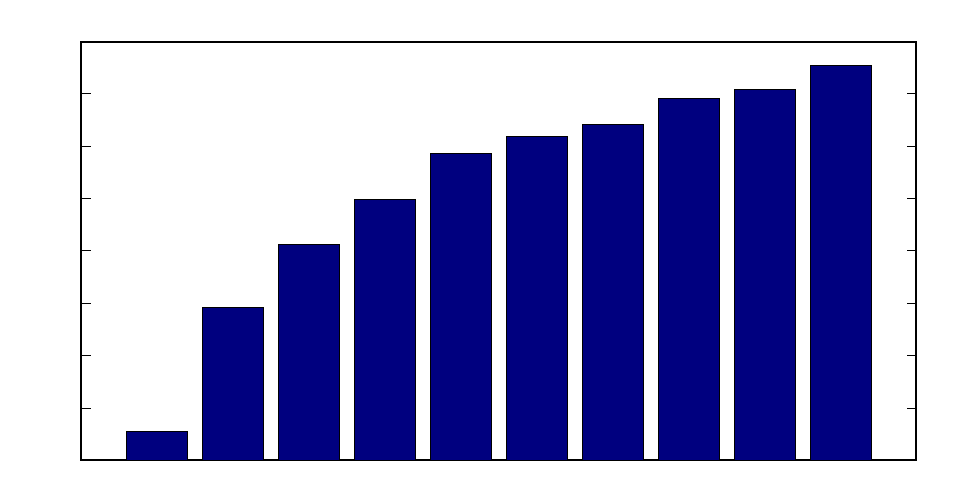
\includegraphics{./imgs/chartBar/starbucks_src_barchart}}%
    \gplfronttext
  \end{picture}%
\endgroup

\vspace{2cm}

\subsubsection{Informaci\'on fuente dst}
A continuaci\'on se muestran las 10 ips con menor cantidad de informaci\'on.

%% GNUPLOT: LaTeX picture with Postscript
\begingroup
  \makeatletter
  \providecommand\color[2][]{%
    \GenericError{(gnuplot) \space\space\space\@spaces}{%
      Package color not loaded in conjunction with
      terminal option `colourtext'%
    }{See the gnuplot documentation for explanation.%
    }{Either use 'blacktext' in gnuplot or load the package
      color.sty in LaTeX.}%
    \renewcommand\color[2][]{}%
  }%
  \providecommand\includegraphics[2][]{%
    \GenericError{(gnuplot) \space\space\space\@spaces}{%
      Package graphicx or graphics not loaded%
    }{See the gnuplot documentation for explanation.%
    }{The gnuplot epslatex terminal needs graphicx.sty or graphics.sty.}%
    \renewcommand\includegraphics[2][]{}%
  }%
  \providecommand\rotatebox[2]{#2}%
  \@ifundefined{ifGPcolor}{%
    \newif\ifGPcolor
    \GPcolorfalse
  }{}%
  \@ifundefined{ifGPblacktext}{%
    \newif\ifGPblacktext
    \GPblacktexttrue
  }{}%
  % define a \g@addto@macro without @ in the name:
  \let\gplgaddtomacro\g@addto@macro
  % define empty templates for all commands taking text:
  \gdef\gplbacktext{}%
  \gdef\gplfronttext{}%
  \makeatother
  \ifGPblacktext
    % no textcolor at all
    \def\colorrgb#1{}%
    \def\colorgray#1{}%
  \else
    % gray or color?
    \ifGPcolor
      \def\colorrgb#1{\color[rgb]{#1}}%
      \def\colorgray#1{\color[gray]{#1}}%
      \expandafter\def\csname LTw\endcsname{\color{white}}%
      \expandafter\def\csname LTb\endcsname{\color{black}}%
      \expandafter\def\csname LTa\endcsname{\color{black}}%
      \expandafter\def\csname LT0\endcsname{\color[rgb]{1,0,0}}%
      \expandafter\def\csname LT1\endcsname{\color[rgb]{0,1,0}}%
      \expandafter\def\csname LT2\endcsname{\color[rgb]{0,0,1}}%
      \expandafter\def\csname LT3\endcsname{\color[rgb]{1,0,1}}%
      \expandafter\def\csname LT4\endcsname{\color[rgb]{0,1,1}}%
      \expandafter\def\csname LT5\endcsname{\color[rgb]{1,1,0}}%
      \expandafter\def\csname LT6\endcsname{\color[rgb]{0,0,0}}%
      \expandafter\def\csname LT7\endcsname{\color[rgb]{1,0.3,0}}%
      \expandafter\def\csname LT8\endcsname{\color[rgb]{0.5,0.5,0.5}}%
    \else
      % gray
      \def\colorrgb#1{\color{black}}%
      \def\colorgray#1{\color[gray]{#1}}%
      \expandafter\def\csname LTw\endcsname{\color{white}}%
      \expandafter\def\csname LTb\endcsname{\color{black}}%
      \expandafter\def\csname LTa\endcsname{\color{black}}%
      \expandafter\def\csname LT0\endcsname{\color{black}}%
      \expandafter\def\csname LT1\endcsname{\color{black}}%
      \expandafter\def\csname LT2\endcsname{\color{black}}%
      \expandafter\def\csname LT3\endcsname{\color{black}}%
      \expandafter\def\csname LT4\endcsname{\color{black}}%
      \expandafter\def\csname LT5\endcsname{\color{black}}%
      \expandafter\def\csname LT6\endcsname{\color{black}}%
      \expandafter\def\csname LT7\endcsname{\color{black}}%
      \expandafter\def\csname LT8\endcsname{\color{black}}%
    \fi
  \fi
  \setlength{\unitlength}{0.0500bp}%
  \begin{picture}(9000.00,4500.00)%
    \gplgaddtomacro\gplbacktext{%
      \colorrgb{0.00,0.00,0.00}%
      \put(620,240){\makebox(0,0)[r]{\strut{}0}}%
      \colorrgb{0.00,0.00,0.00}%
      \put(620,1044){\makebox(0,0)[r]{\strut{}2}}%
      \colorrgb{0.00,0.00,0.00}%
      \put(620,1848){\makebox(0,0)[r]{\strut{}4}}%
      \colorrgb{0.00,0.00,0.00}%
      \put(620,2651){\makebox(0,0)[r]{\strut{}6}}%
      \colorrgb{0.00,0.00,0.00}%
      \put(620,3455){\makebox(0,0)[r]{\strut{}8}}%
      \colorrgb{0.00,0.00,0.00}%
      \put(620,4259){\makebox(0,0)[r]{\strut{}10}}%
      \colorrgb{0.00,0.00,0.00}%
      \put(160,2249){\rotatebox{90}{\makebox(0,0){\strut{}Informaci\'on}}}%
    }%
    \gplgaddtomacro\gplfronttext{%
      \colorrgb{0.00,0.00,0.00}%
      \put(1458,29){\rotatebox{45}{\makebox(0,0)[r]{\strut{}10.254.54.1}}}%
      \put(2176,29){\rotatebox{45}{\makebox(0,0)[r]{\strut{}10.254.54.216}}}%
      \put(2894,29){\rotatebox{45}{\makebox(0,0)[r]{\strut{}10.254.54.251}}}%
      \put(3612,29){\rotatebox{45}{\makebox(0,0)[r]{\strut{}10.254.54.248}}}%
      \put(4330,29){\rotatebox{45}{\makebox(0,0)[r]{\strut{}10.254.54.6}}}%
      \put(5049,29){\rotatebox{45}{\makebox(0,0)[r]{\strut{}10.254.54.115}}}%
      \put(5767,29){\rotatebox{45}{\makebox(0,0)[r]{\strut{}10.254.54.226}}}%
      \put(6485,29){\rotatebox{45}{\makebox(0,0)[r]{\strut{}10.254.54.12}}}%
      \put(7203,29){\rotatebox{45}{\makebox(0,0)[r]{\strut{}10.254.54.149}}}%
      \put(7921,29){\rotatebox{45}{\makebox(0,0)[r]{\strut{}10.254.54.138}}}%
    }%
    \gplbacktext
    \put(0,0){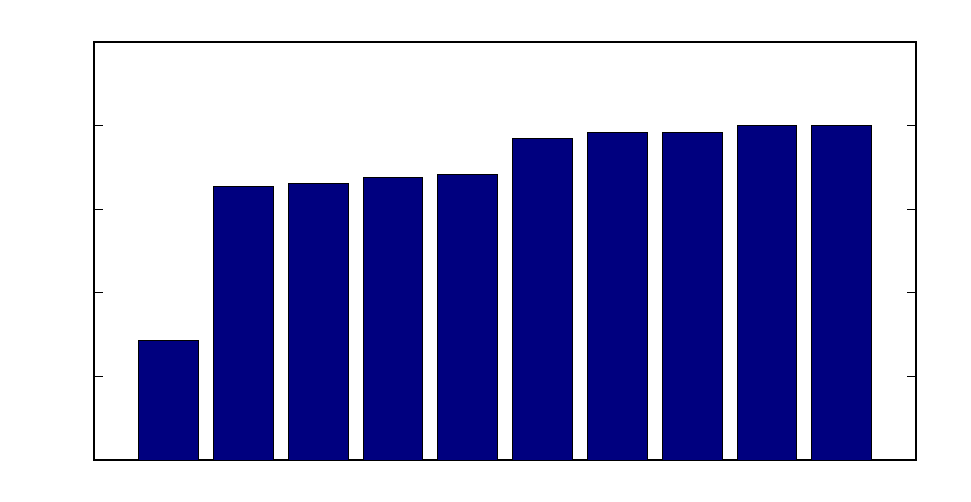
\includegraphics{./imgs/chartBar/starbucks_dst_barchart}}%
    \gplfronttext
  \end{picture}%
\endgroup

\vspace{2cm}


\subsubsection{Informaci\'on fuente src}
A continuaci\'on se muestran las 10 ips con menor cantidad de informaci\'on.

%% GNUPLOT: LaTeX picture with Postscript
\begingroup
  \makeatletter
  \providecommand\color[2][]{%
    \GenericError{(gnuplot) \space\space\space\@spaces}{%
      Package color not loaded in conjunction with
      terminal option `colourtext'%
    }{See the gnuplot documentation for explanation.%
    }{Either use 'blacktext' in gnuplot or load the package
      color.sty in LaTeX.}%
    \renewcommand\color[2][]{}%
  }%
  \providecommand\includegraphics[2][]{%
    \GenericError{(gnuplot) \space\space\space\@spaces}{%
      Package graphicx or graphics not loaded%
    }{See the gnuplot documentation for explanation.%
    }{The gnuplot epslatex terminal needs graphicx.sty or graphics.sty.}%
    \renewcommand\includegraphics[2][]{}%
  }%
  \providecommand\rotatebox[2]{#2}%
  \@ifundefined{ifGPcolor}{%
    \newif\ifGPcolor
    \GPcolorfalse
  }{}%
  \@ifundefined{ifGPblacktext}{%
    \newif\ifGPblacktext
    \GPblacktexttrue
  }{}%
  % define a \g@addto@macro without @ in the name:
  \let\gplgaddtomacro\g@addto@macro
  % define empty templates for all commands taking text:
  \gdef\gplbacktext{}%
  \gdef\gplfronttext{}%
  \makeatother
  \ifGPblacktext
    % no textcolor at all
    \def\colorrgb#1{}%
    \def\colorgray#1{}%
  \else
    % gray or color?
    \ifGPcolor
      \def\colorrgb#1{\color[rgb]{#1}}%
      \def\colorgray#1{\color[gray]{#1}}%
      \expandafter\def\csname LTw\endcsname{\color{white}}%
      \expandafter\def\csname LTb\endcsname{\color{black}}%
      \expandafter\def\csname LTa\endcsname{\color{black}}%
      \expandafter\def\csname LT0\endcsname{\color[rgb]{1,0,0}}%
      \expandafter\def\csname LT1\endcsname{\color[rgb]{0,1,0}}%
      \expandafter\def\csname LT2\endcsname{\color[rgb]{0,0,1}}%
      \expandafter\def\csname LT3\endcsname{\color[rgb]{1,0,1}}%
      \expandafter\def\csname LT4\endcsname{\color[rgb]{0,1,1}}%
      \expandafter\def\csname LT5\endcsname{\color[rgb]{1,1,0}}%
      \expandafter\def\csname LT6\endcsname{\color[rgb]{0,0,0}}%
      \expandafter\def\csname LT7\endcsname{\color[rgb]{1,0.3,0}}%
      \expandafter\def\csname LT8\endcsname{\color[rgb]{0.5,0.5,0.5}}%
    \else
      % gray
      \def\colorrgb#1{\color{black}}%
      \def\colorgray#1{\color[gray]{#1}}%
      \expandafter\def\csname LTw\endcsname{\color{white}}%
      \expandafter\def\csname LTb\endcsname{\color{black}}%
      \expandafter\def\csname LTa\endcsname{\color{black}}%
      \expandafter\def\csname LT0\endcsname{\color{black}}%
      \expandafter\def\csname LT1\endcsname{\color{black}}%
      \expandafter\def\csname LT2\endcsname{\color{black}}%
      \expandafter\def\csname LT3\endcsname{\color{black}}%
      \expandafter\def\csname LT4\endcsname{\color{black}}%
      \expandafter\def\csname LT5\endcsname{\color{black}}%
      \expandafter\def\csname LT6\endcsname{\color{black}}%
      \expandafter\def\csname LT7\endcsname{\color{black}}%
      \expandafter\def\csname LT8\endcsname{\color{black}}%
    \fi
  \fi
  \setlength{\unitlength}{0.0500bp}%
  \begin{picture}(9000.00,4500.00)%
    \gplgaddtomacro\gplbacktext{%
      \colorrgb{0.00,0.00,0.00}%
      \put(500,240){\makebox(0,0)[r]{\strut{}0}}%
      \colorrgb{0.00,0.00,0.00}%
      \put(500,1044){\makebox(0,0)[r]{\strut{}1}}%
      \colorrgb{0.00,0.00,0.00}%
      \put(500,1848){\makebox(0,0)[r]{\strut{}2}}%
      \colorrgb{0.00,0.00,0.00}%
      \put(500,2651){\makebox(0,0)[r]{\strut{}3}}%
      \colorrgb{0.00,0.00,0.00}%
      \put(500,3455){\makebox(0,0)[r]{\strut{}4}}%
      \colorrgb{0.00,0.00,0.00}%
      \put(500,4259){\makebox(0,0)[r]{\strut{}5}}%
      \colorrgb{0.00,0.00,0.00}%
      \put(160,2249){\rotatebox{90}{\makebox(0,0){\strut{}Informaci\'on}}}%
    }%
    \gplgaddtomacro\gplfronttext{%
      \colorrgb{0.00,0.00,0.00}%
      \put(1349,29){\rotatebox{45}{\makebox(0,0)[r]{\strut{}192.168.1.46}}}%
      \put(2078,29){\rotatebox{45}{\makebox(0,0)[r]{\strut{}192.168.1.22}}}%
      \put(2807,29){\rotatebox{45}{\makebox(0,0)[r]{\strut{}192.168.1.36}}}%
      \put(3536,29){\rotatebox{45}{\makebox(0,0)[r]{\strut{}192.168.1.15}}}%
      \put(4265,29){\rotatebox{45}{\makebox(0,0)[r]{\strut{}192.168.1.42}}}%
      \put(4994,29){\rotatebox{45}{\makebox(0,0)[r]{\strut{}192.168.1.6}}}%
      \put(5723,29){\rotatebox{45}{\makebox(0,0)[r]{\strut{}192.168.1.1}}}%
      \put(6452,29){\rotatebox{45}{\makebox(0,0)[r]{\strut{}0.0.0.0}}}%
      \put(7181,29){\rotatebox{45}{\makebox(0,0)[r]{\strut{}192.168.1.8}}}%
      \put(7910,29){\rotatebox{45}{\makebox(0,0)[r]{\strut{}192.168.1.28}}}%
    }%
    \gplbacktext
    \put(0,0){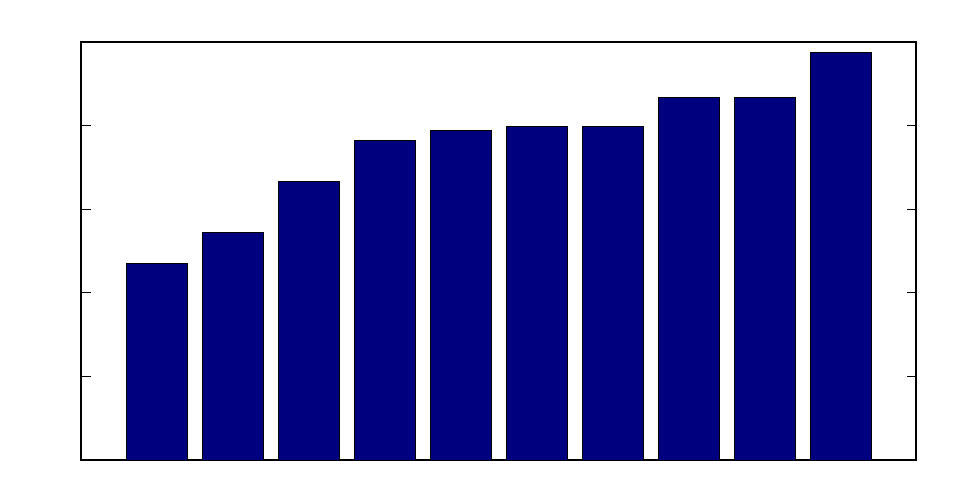
\includegraphics{./imgs/chartBar/tiarg_src_barchart}}%
    \gplfronttext
  \end{picture}%
\endgroup

\vspace{2cm}

\subsubsection{Informaci\'on fuente dst}
A continuaci\'on se muestran las 10 ips con menor cantidad de informaci\'on.

%% GNUPLOT: LaTeX picture with Postscript
\begingroup
  \makeatletter
  \providecommand\color[2][]{%
    \GenericError{(gnuplot) \space\space\space\@spaces}{%
      Package color not loaded in conjunction with
      terminal option `colourtext'%
    }{See the gnuplot documentation for explanation.%
    }{Either use 'blacktext' in gnuplot or load the package
      color.sty in LaTeX.}%
    \renewcommand\color[2][]{}%
  }%
  \providecommand\includegraphics[2][]{%
    \GenericError{(gnuplot) \space\space\space\@spaces}{%
      Package graphicx or graphics not loaded%
    }{See the gnuplot documentation for explanation.%
    }{The gnuplot epslatex terminal needs graphicx.sty or graphics.sty.}%
    \renewcommand\includegraphics[2][]{}%
  }%
  \providecommand\rotatebox[2]{#2}%
  \@ifundefined{ifGPcolor}{%
    \newif\ifGPcolor
    \GPcolorfalse
  }{}%
  \@ifundefined{ifGPblacktext}{%
    \newif\ifGPblacktext
    \GPblacktexttrue
  }{}%
  % define a \g@addto@macro without @ in the name:
  \let\gplgaddtomacro\g@addto@macro
  % define empty templates for all commands taking text:
  \gdef\gplbacktext{}%
  \gdef\gplfronttext{}%
  \makeatother
  \ifGPblacktext
    % no textcolor at all
    \def\colorrgb#1{}%
    \def\colorgray#1{}%
  \else
    % gray or color?
    \ifGPcolor
      \def\colorrgb#1{\color[rgb]{#1}}%
      \def\colorgray#1{\color[gray]{#1}}%
      \expandafter\def\csname LTw\endcsname{\color{white}}%
      \expandafter\def\csname LTb\endcsname{\color{black}}%
      \expandafter\def\csname LTa\endcsname{\color{black}}%
      \expandafter\def\csname LT0\endcsname{\color[rgb]{1,0,0}}%
      \expandafter\def\csname LT1\endcsname{\color[rgb]{0,1,0}}%
      \expandafter\def\csname LT2\endcsname{\color[rgb]{0,0,1}}%
      \expandafter\def\csname LT3\endcsname{\color[rgb]{1,0,1}}%
      \expandafter\def\csname LT4\endcsname{\color[rgb]{0,1,1}}%
      \expandafter\def\csname LT5\endcsname{\color[rgb]{1,1,0}}%
      \expandafter\def\csname LT6\endcsname{\color[rgb]{0,0,0}}%
      \expandafter\def\csname LT7\endcsname{\color[rgb]{1,0.3,0}}%
      \expandafter\def\csname LT8\endcsname{\color[rgb]{0.5,0.5,0.5}}%
    \else
      % gray
      \def\colorrgb#1{\color{black}}%
      \def\colorgray#1{\color[gray]{#1}}%
      \expandafter\def\csname LTw\endcsname{\color{white}}%
      \expandafter\def\csname LTb\endcsname{\color{black}}%
      \expandafter\def\csname LTa\endcsname{\color{black}}%
      \expandafter\def\csname LT0\endcsname{\color{black}}%
      \expandafter\def\csname LT1\endcsname{\color{black}}%
      \expandafter\def\csname LT2\endcsname{\color{black}}%
      \expandafter\def\csname LT3\endcsname{\color{black}}%
      \expandafter\def\csname LT4\endcsname{\color{black}}%
      \expandafter\def\csname LT5\endcsname{\color{black}}%
      \expandafter\def\csname LT6\endcsname{\color{black}}%
      \expandafter\def\csname LT7\endcsname{\color{black}}%
      \expandafter\def\csname LT8\endcsname{\color{black}}%
    \fi
  \fi
  \setlength{\unitlength}{0.0500bp}%
  \begin{picture}(9000.00,4500.00)%
    \gplgaddtomacro\gplbacktext{%
      \colorrgb{0.00,0.00,0.00}%
      \put(500,240){\makebox(0,0)[r]{\strut{}0}}%
      \colorrgb{0.00,0.00,0.00}%
      \put(500,910){\makebox(0,0)[r]{\strut{}1}}%
      \colorrgb{0.00,0.00,0.00}%
      \put(500,1580){\makebox(0,0)[r]{\strut{}2}}%
      \colorrgb{0.00,0.00,0.00}%
      \put(500,2250){\makebox(0,0)[r]{\strut{}3}}%
      \colorrgb{0.00,0.00,0.00}%
      \put(500,2919){\makebox(0,0)[r]{\strut{}4}}%
      \colorrgb{0.00,0.00,0.00}%
      \put(500,3589){\makebox(0,0)[r]{\strut{}5}}%
      \colorrgb{0.00,0.00,0.00}%
      \put(500,4259){\makebox(0,0)[r]{\strut{}6}}%
      \colorrgb{0.00,0.00,0.00}%
      \put(160,2249){\rotatebox{90}{\makebox(0,0){\strut{}Informaci\'on}}}%
    }%
    \gplgaddtomacro\gplfronttext{%
      \colorrgb{0.00,0.00,0.00}%
      \put(1349,29){\rotatebox{45}{\makebox(0,0)[r]{\strut{}192.168.1.1}}}%
      \put(2078,29){\rotatebox{45}{\makebox(0,0)[r]{\strut{}192.168.1.15}}}%
      \put(2807,29){\rotatebox{45}{\makebox(0,0)[r]{\strut{}192.168.1.32}}}%
      \put(3536,29){\rotatebox{45}{\makebox(0,0)[r]{\strut{}192.168.1.5}}}%
      \put(4265,29){\rotatebox{45}{\makebox(0,0)[r]{\strut{}192.168.1.13}}}%
      \put(4994,29){\rotatebox{45}{\makebox(0,0)[r]{\strut{}192.168.1.6}}}%
      \put(5723,29){\rotatebox{45}{\makebox(0,0)[r]{\strut{}192.168.1.64}}}%
      \put(6452,29){\rotatebox{45}{\makebox(0,0)[r]{\strut{}192.168.1.22}}}%
      \put(7181,29){\rotatebox{45}{\makebox(0,0)[r]{\strut{}192.168.1.29}}}%
      \put(7910,29){\rotatebox{45}{\makebox(0,0)[r]{\strut{}192.168.1.28}}}%
    }%
    \gplbacktext
    \put(0,0){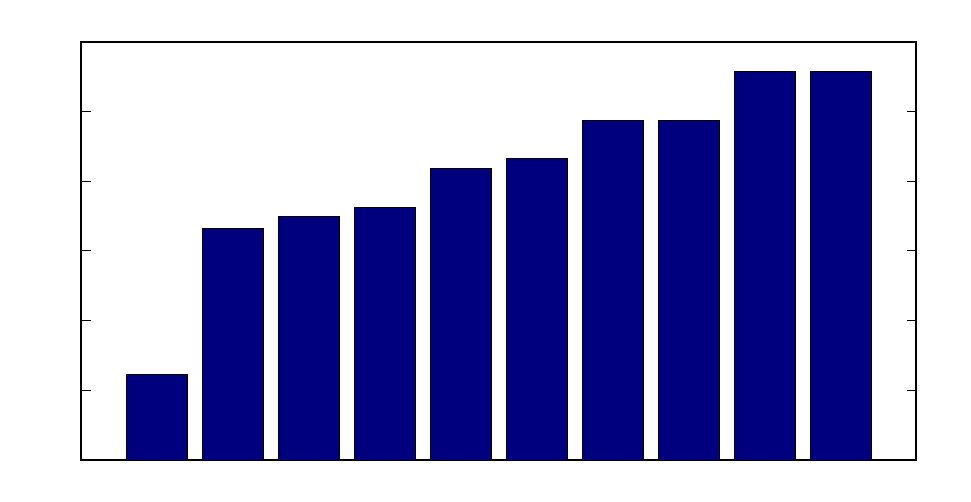
\includegraphics{./imgs/chartBar/tiarg_dst_barchart}}%
    \gplfronttext
  \end{picture}%
\endgroup

\vspace{2cm}

\section{Referencias}
\begin{itemize}
\item PETERSON, DAVIE ; Computer Networks, 5th edition, Wiley
\item STEVENS, W. Richard ; TCP/IP Illustrated, Volume 1

\item $http://wiki.wireshark.org/Gratuitous\_ARP$
\end{itemize}
\end{document}
